%!TeX root = safety
\documentclass[paper.tex]{subfiles}
\begin{document}

\clearpage
%%%%%%%%%%%%%%%%%%%%%%%%%%%%%%%%%%%%%%%%%%%%%%%%
\begin{multicols}{1}
{\Large Safety}\\
%%%%%%%%%%%%%%%%%%%%%%%%%%%%%%%%%%%%%%%%%%%%%%%%

One could subsist on non-thermal effects literature alone. There is drama, mystery, intrigue, paragraphs of sardonic ire; ad-hominem analogies; effects spanning 10 orders of magnitude in strength and scale; where the tiniest of atomic murmurs sparks.

The picture is certainly much more complicated than "non-ionizing cannot have effects".



Because this is an ostensibly novel and niche mechanism, it may behoove us to briefly review the biological basis for the safety limits set by standards organizations. \footnote{The idea of biological microwave resonances appears to have originated in [Frohlich 1968, 1980].}


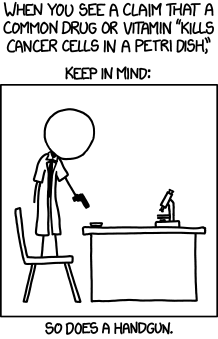
\includegraphics[scale=0.5]{cells.png}


There are also things.

For instance, it is reasonable to wonder why we might not see such resonances in bodily tissues. Approximately similar nanoscopic structures exist in humans, such as nuclear pores (120 nm) and the famous microtubules (10x50 nm). 

While from which epidemiological data could be derived.\footnote{The cloud service [scite.ai] was useful during this review.}

What we find is a messy affair. Biology is hard.

\rule{\linewidth}{0.2pt}

There are some 20,000 papers on the topic of RF safety, with solid in vitro, in vivo and epidemiological evidence of safety in the 2.4 GHz and 5.8 GHz bands.

However, "There are limited experimental human data upon which to set limits on exposures above 6 GHz" [Chan 2019]. Only 2\% of the above papers are on frequencies $>6$ GHz [Vijayalaxmi 2018]. 

In addition, what data remains in this category is of varying quality. 

As has been starkly demonstrated in the recent hydroxychloroquine contradictions [Gautret 2020] [Geleris 2020], biological research must be essentially perfect to have any meaning at all.


The IEEE standard which the flagship paper [Yang 2015] references [IEEE C95.1-2005] was recently overhauled [IEEE C95.1-2019] with new metrics.


[Vijayalaxmi 2018] is a remarkable meta-analysis of in vitro data. They synthesize a quality score, rating bindedness, sham controls, dosimetry, and sample size. Quality was inversely, monotonically related to the effect size. An example of the subtle effects that can call into question superfically reasonable results are [

They additionally find a publication bias of incredible magnitude in the positive (harm) direction in this field, further degrading the usefulness of statistical analyeses.

An example of a relevant study that they grade as "quality 1" [Karaca 2011]. This study's conclusion is that However, in figure 5, one can see that only 1 out of 11 genes tested had a statistically significant difference in expression. Given the N=6 cultures, 

\rule{\linewidth}{0.2pt}

[Adair 2002] demonstrate theoretically that acoustic resonances are, in general, highly unlikely in biological solvents, primarily focusing on DNA. All resonance modes are strongly overdamped by the surrounding solvent, and no amplitude amplification can take place.

This analysis would seem to disagree with the viral resonance apparently conclusively demonstrated by [Yang 2015] - the PCR result seems especially inarguable. This could be explained by the large charge on the virus compared to the molecules analyzed in Adair. [Yang 2015] find a charge of order $10^7 e$, whereas Adair analyzes a very different regime, "assume coupling to the field through single charges q = e at each end".

[Liu 2009] cite [Edwards, Swicord 1984], saying: "It was proposed that a hydration layer surrounding DNA molecules could lower the viscoelastic transition
frequency, raise the quality factor of confined acoustic vibrations, and result in a microwave resonant absorption". 

But [Adair 2002]'s [Foster 1987] seem to quite conclusively put the kibosh on that idea, demonstrating no resonances in DNA with 20x higher precision than previous work, showing previous results to be an artifact of the measurement equipment.

The supplemental material to [Vijayalaxmi 2018] has a table of studies on this topic. High-quality research in-vitro concurs with.

\paragraph{[Manikowska 1979]} \

9.4 GHz pulsed / in vivo, mouse, $0.1-10 \text{mW}/\text{m}^2$ over the whole body for 2 weeks. N=16.

This is a particularly concerning result, especially given their $p<0.001$. [Servantie 1989] discusses the (admittedly circuituious) route by which birth defects could occur.

Work by [Manikowska 1985] in the 2.4 GHz range has been contradicted [Beechey 1986], but the 9 GHz range does not appear to have been repeated.

\rule{\linewidth}{0.2pt}

More modern research [Juutilainen 2011], [Chemeris], [Vijayalaxmi 2006],  does not tend to agree with these concerns. As cited by [ICNIRP 2020]'s excellent literature review, expose lymphocyte blood cells to 8 ns pulsed 8.2 GHz radiation for 2 hours at an average power of $10 \text{mW/cm}^2$. They find no change in any of the parameters measured, including various chromosomal parameters. They further discuss previous results.

\rule{\linewidth}{0.2pt}

In the frequency range of interest, there seems to be good-quality in-vitro evidence using lymphocytes of lack of harm. We are not aware of any high-quality in vivo or epidemeological data from which useful conclusions can be drawn. 

We must defer to health experts for interpretation of these data.

\rule{\linewidth}{0.2pt}

{\it Please contact the author if you are aware of other salient research, or have a different interpretation.}

\end{multicols}



\end{document}
